% NeurIPS 2026 poster -- Overleaf-friendly beamerposter source
% Size: 36 in x 24 in landscape (91.44 cm x 60.96 cm)
% Compiler: pdfLaTeX (Overleaf default)
% Main file: neurips_poster.tex  |  keep figures/ next to this file

\documentclass[final,t]{beamer}

% Do NOT load hyperref or geometry yourself -- beamer / beamerposter already do.
\usepackage[size=custom,width=91.44,height=60.96,scale=0.88]{beamerposter}
\usepackage[T1]{fontenc}
\usepackage{lmodern}
\usepackage{booktabs}
\usepackage{array}
\usepackage{amsmath,amssymb}
\usepackage{tikz}
\usepackage{ragged2e}

% Optional QR (Overleaf has qrcode; local installs may not).
\IfFileExists{qrcode.sty}{%
  \usepackage{qrcode}%
  \newcommand{\ProjectQR}{\qrcode[height=2.0cm]{https://cent664.github.io/LLMID/}}%
}{%
  \newcommand{\ProjectQR}{%
    \fbox{\parbox[c][2.0cm][c]{2.0cm}{\centering\scriptsize
      Project page\\[0.15em]\texttt{cent664.github.io/LLMID}}}}%
}

% Theme colors (match project page)
\definecolor{Ink}{HTML}{101820}
\definecolor{Muted}{HTML}{5A6A78}
\definecolor{Accent}{HTML}{0E7C86}
\definecolor{AccentDeep}{HTML}{0A5F67}
\definecolor{Signal}{HTML}{C45C26}
\definecolor{Paper}{HTML}{F2F6F8}
\definecolor{Panel}{HTML}{FFFFFF}
\definecolor{Line}{HTML}{D5DFE6}

\setbeamercolor{background canvas}{bg=Paper}
\setbeamercolor{normal text}{fg=Ink}
\setbeamercolor{block title}{fg=AccentDeep,bg=Panel}
\setbeamercolor{block body}{fg=Ink,bg=Panel}
\setbeamerfont{block title}{series=\bfseries,size=\large}
\setbeamerfont{block body}{size=\normalsize}
\setbeamertemplate{navigation symbols}{}

% Simple block chrome (no custom beamercolorbox options that break on Overleaf)
\setbeamertemplate{block begin}{%
  \vspace{0.2em}%
  \begin{beamercolorbox}[colsep*=0.4ex,leftskip=0.4em,rightskip=0.4em]{block title}%
    \usebeamerfont{block title}\insertblocktitle
  \end{beamercolorbox}%
  {\color{Accent}\hrule height 1.2pt}%
  \begin{beamercolorbox}[colsep*=0.5ex,leftskip=0.4em,rightskip=0.4em]{block body}%
    \justifying\usebeamerfont{block body}\vspace{0.1em}%
}
\setbeamertemplate{block end}{%
  \end{beamercolorbox}%
  \vspace{0.2em}%
}

\newcommand{\TinyCap}[1]{{\scriptsize\color{Muted}#1}}
\newcommand{\Key}[1]{\textbf{\color{AccentDeep}#1}}

\title{Invariant Features in Language Models}
\author{Agnibh Dasgupta, Abdullah All Tanvir, Xin Zhong}
\institute{University of Nebraska Omaha}

\begin{document}
\begin{frame}[t,fragile]

% ----- Header -----
{\scriptsize\color{Accent}\textbf{NEURIPS 2026 -- POSTER}}
\hfill
{\scriptsize\color{Muted}%
  arXiv:2605.06458 -- cs.LG \quad|\quad
  \href{https://cent664.github.io/LLMID/}{\color{Accent}cent664.github.io/LLMID}}

\vspace{0.15em}
{\LARGE\bfseries\color{Ink} Invariant Features in Language Models: Geometric Characterization and Model Attribution}

\vspace{0.15em}
{\normalsize Agnibh Dasgupta$^{*}$, Abdullah All Tanvir$^{*}$, Xin Zhong$^{\dagger}$
\quad{\small\color{Muted}$^{*}$Equal contribution. $^{\dagger}$Corresponding author.
\quad University of Nebraska Omaha.}}

\vspace{0.25em}
{\color{Line}\hrule height 1pt}
\vspace{0.3em}

% ----- Body -----
\begin{columns}[t,onlytextwidth]

% LEFT
\begin{column}{0.31\textwidth}

\begin{block}{TL;DR}
We give a \Key{local geometric characterization} of semantic invariance:
paraphrases tend to move along nuisance directions, while meaning lives in a
more stable subspace. Contrasting meaning-preserving and meaning-changing edits
recovers that subspace. Interventions test it, and its model-specific geometry
supports \Key{zero-shot model attribution}.
\end{block}

\begin{block}{Problem}
Language models answer paraphrases consistently, suggesting stable meaning
codes. A raw hidden state mixes meaning with surface form: paraphrases can sit
far apart while different questions sit close together. Prior work finds
semantic structure, but does not separate meaning-preserving (SP) from
meaning-changing (SC) variation.

\vspace{0.25em}
\Key{Questions.} Where does a stable semantic subspace exist? How do we find
it? Does it differ across models?
\end{block}

\begin{block}{Dataset}
\begin{tabular}{@{}ll@{}}
Semantic groups & 1{,}400 \\
Domains & 13 \\
Sentences & 57{,}400 \\
Per group & 1 anchor, 20 SP, 10 soft SC, 10 hard SC \\
Split & Disjoint discovery / validation \\
\end{tabular}

\vspace{0.3em}
\TinyCap{Example (France). Anchor: official language of France.
SP: paraphrase. Soft SC: capital of France. Hard SC: longest river in South America.}
\end{block}

\begin{block}{Method (three steps)}
\textbf{1. Local geometric definition.}
Invariant features stay stable under meaning-preserving edits and still
distinguish meanings; locally, the tangent space splits into semantic and nuisance directions.

\vspace{0.15em}
\textbf{2. Contrastive sensitivity decomposition.}
From SP/SC hidden-state changes, form $S_{\mathrm{SP}}$, $S_{\mathrm{SC}}$ and solve
\[
S_{\mathrm{SC}}\,v=\lambda\,(S_{\mathrm{SP}}+\varepsilon I)\,v.
\]
Large-$\lambda$ directions vary under meaning changes, little under paraphrases.
Top-$k$ = invariant; complement = nuisance: $z=z_{\mathrm{inv}}+z_{\mathrm{nuis}}$.

\vspace{0.15em}
\textbf{3. Zero-shot attribution.}
Concatenate invariant projections from the strongest-separation layers
(the invariant zone) into a model signature; match the nearest reference.
\end{block}

\end{column}

% MIDDLE
\begin{column}{0.355\textwidth}

\begin{block}{Overview}
\centering
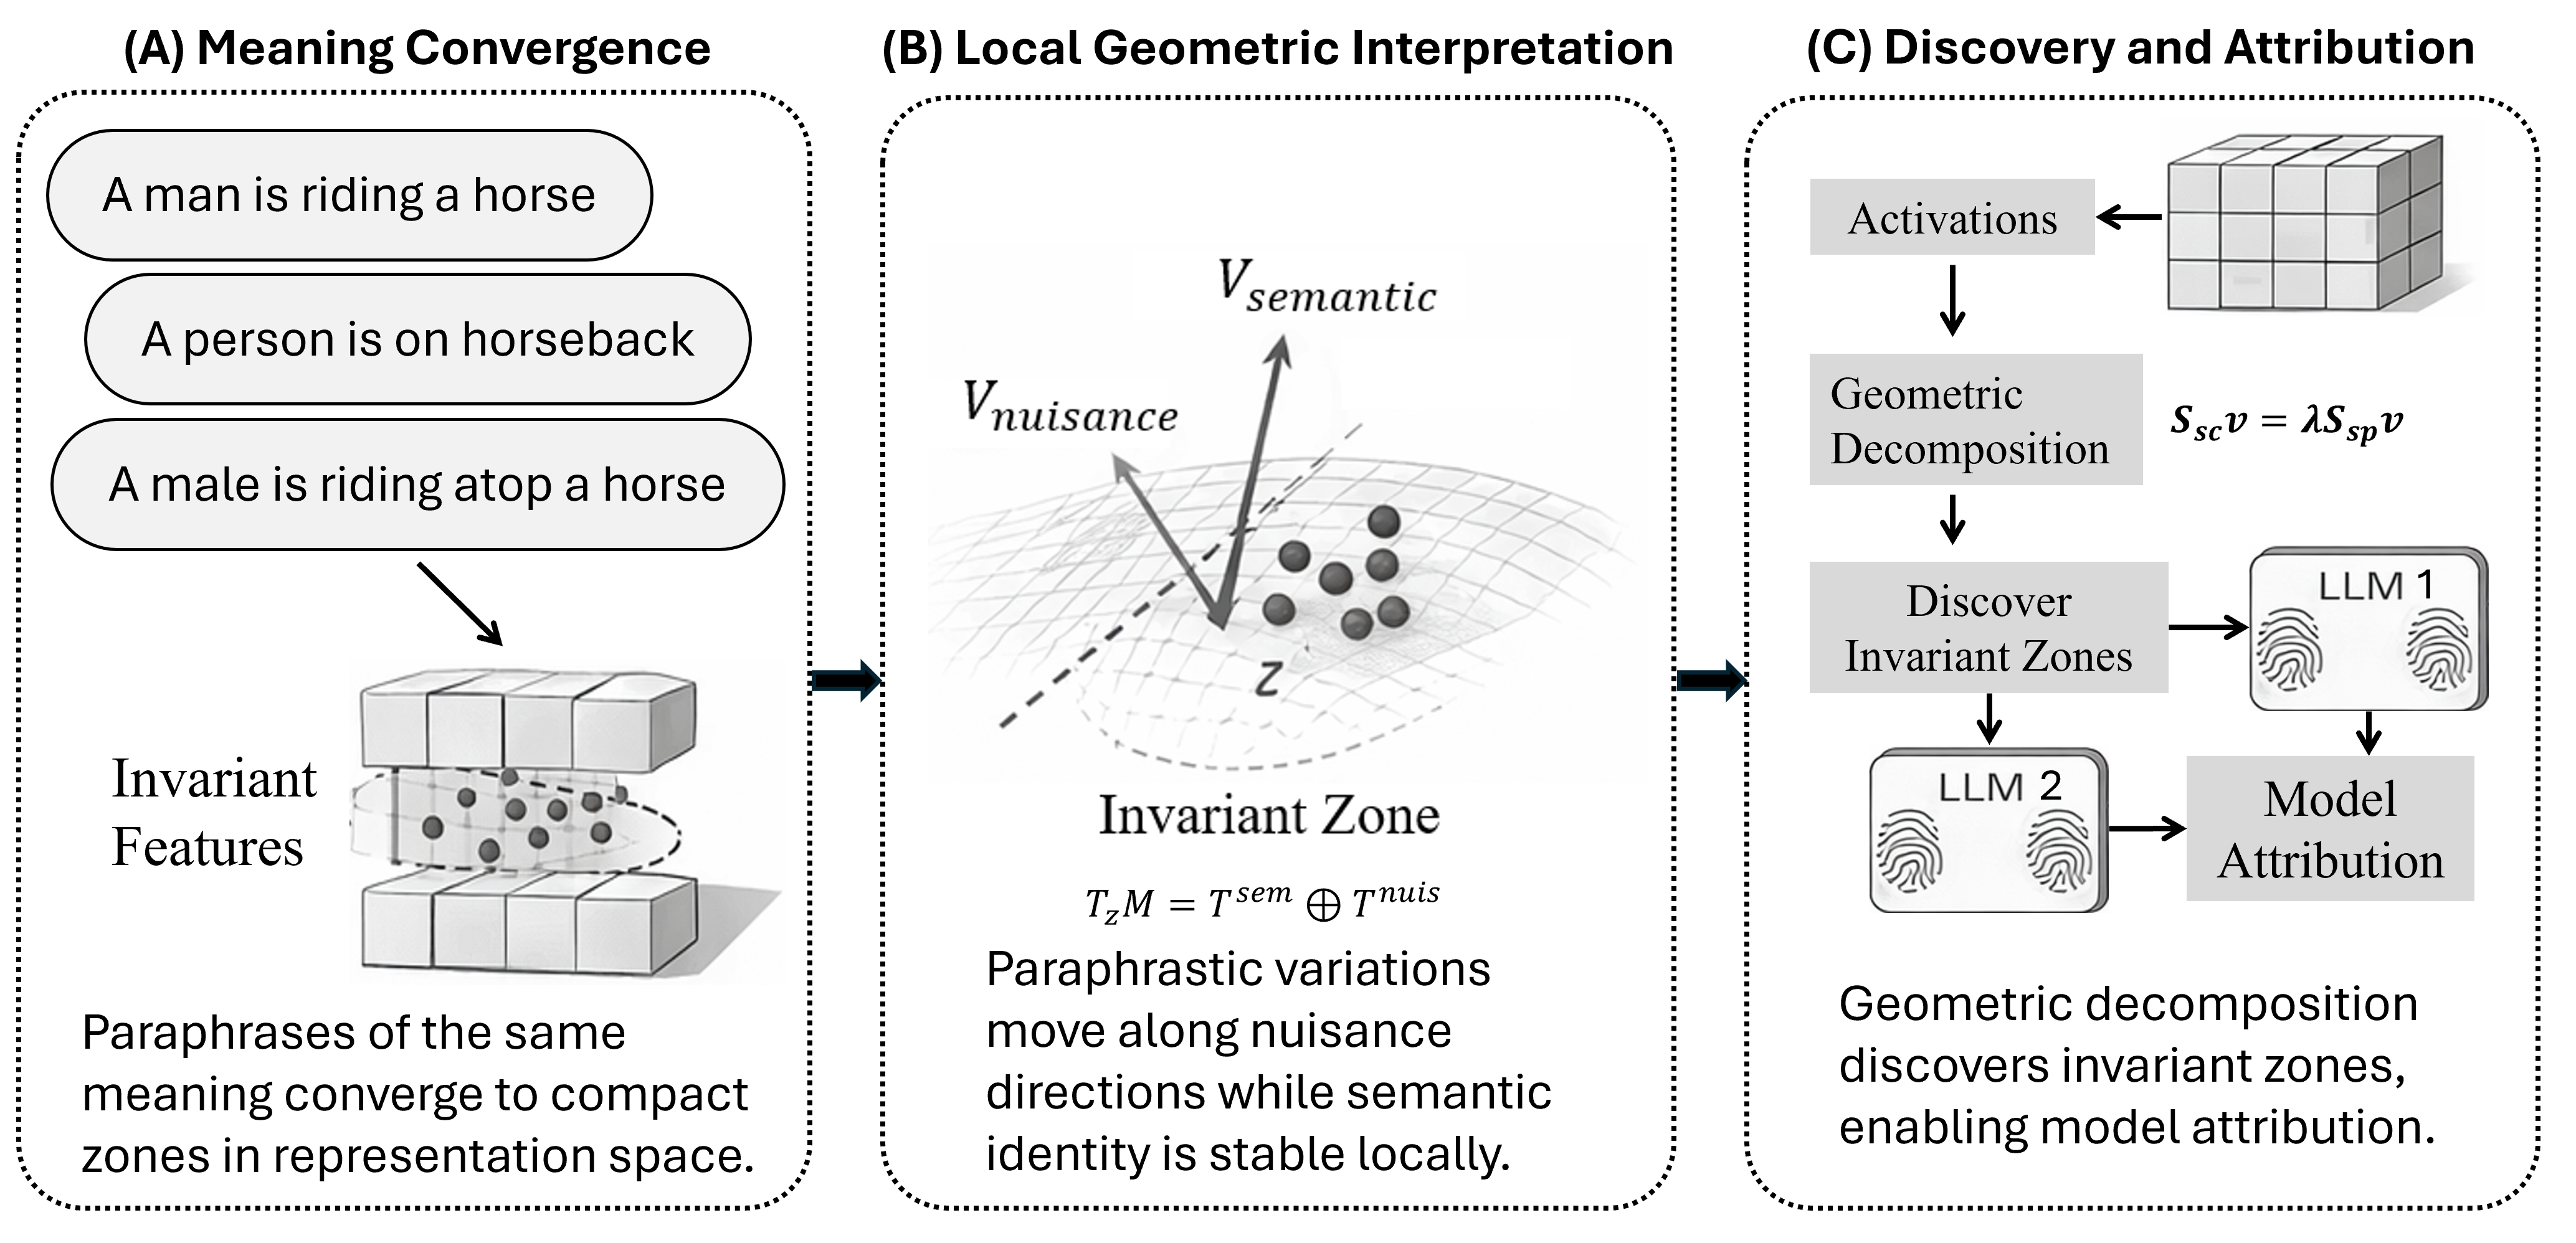
\includegraphics[width=0.92\linewidth]{figures/1_PIA.png}\\
\TinyCap{Fig.~1. (A) Paraphrases converge to compact zones. (B) Nuisance vs semantic directions.
(C) Invariant zones for model attribution.}
\end{block}

\begin{block}{Local geometry and attribution}
\centering
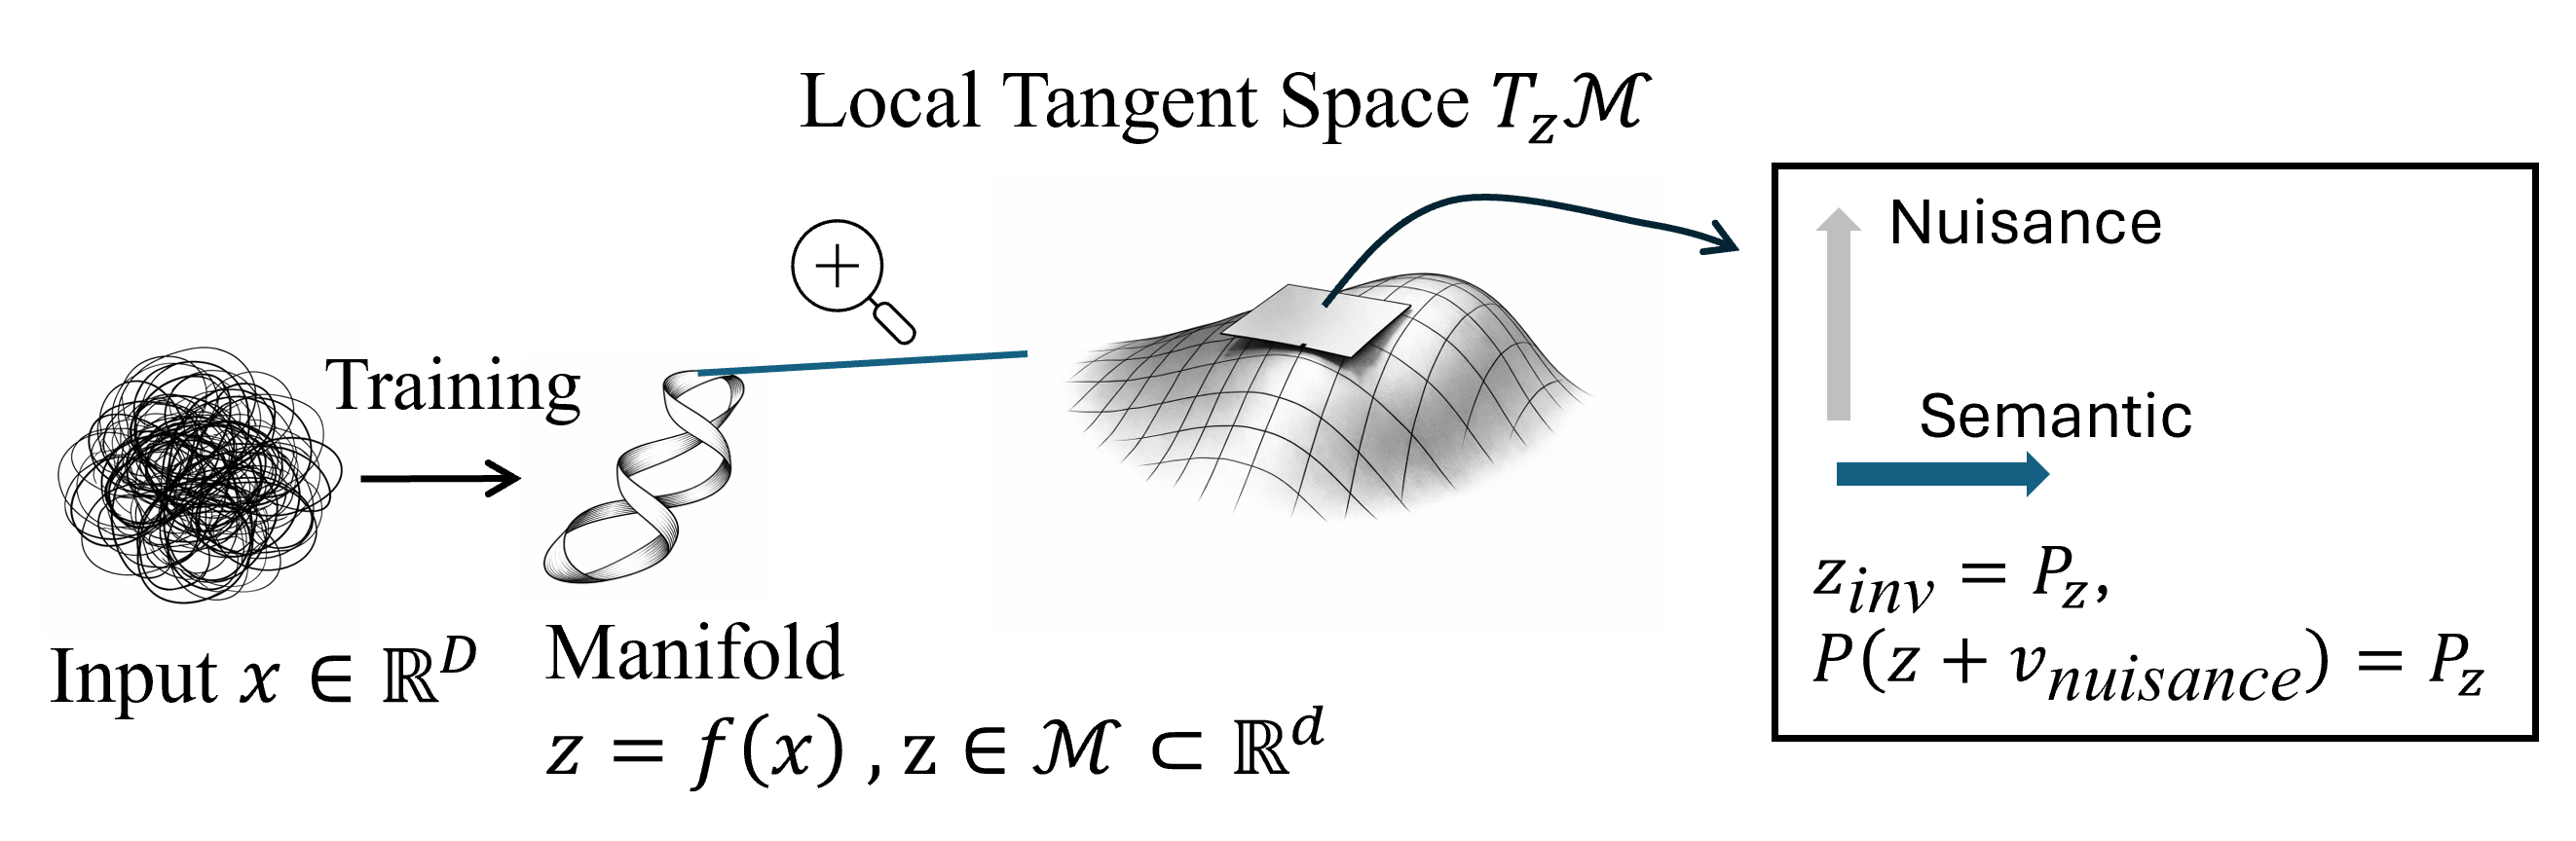
\includegraphics[width=0.92\linewidth]{figures/2_Define.png}\\
\TinyCap{Fig.~2. Local geometric hypothesis: project away nuisance motion.}

\vspace{0.15em}
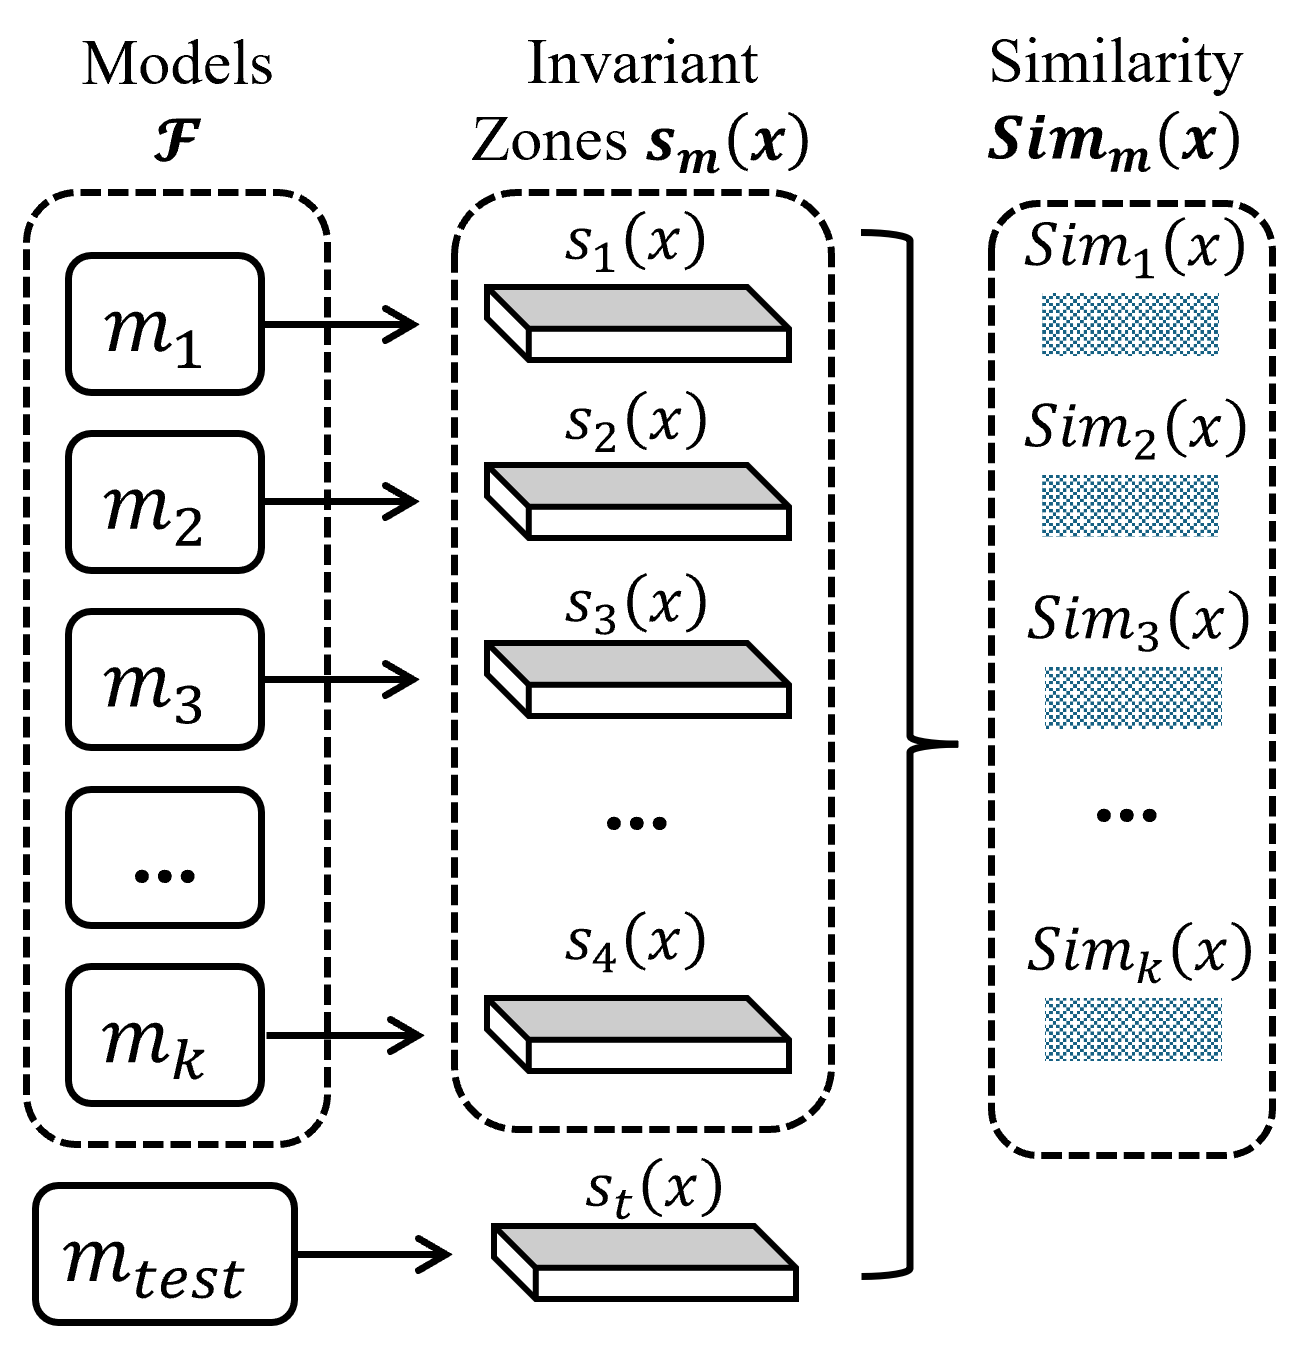
\includegraphics[width=0.48\linewidth]{figures/3_Attribution.png}\\
\TinyCap{Fig.~3. Match invariant-zone signatures across reference models.}
\end{block}

\begin{block}{Meaning outside the nuisance subspace}
$E_{\mathrm{nuis}}$ is the fraction of displacement between two group centroids
that lies in the nuisance subspace. On Llama, our subspace yields much lower
layerwise $E_{\mathrm{nuis}}$ than PCA or cPCA (Table~12).

\vspace{0.25em}
\centering
\begin{tabular}{lccc}
\toprule
Layer & Ours $\downarrow$ & cPCA & PCA \\
\midrule
1  & \textbf{0.0025} & 0.0323 & 0.7320 \\
4  & \textbf{0.0050} & 0.0676 & 0.5584 \\
8  & \textbf{0.0085} & 0.0691 & 0.8851 \\
12 & \textbf{0.0053} & 0.0590 & 0.9572 \\
16 & \textbf{0.0047} & 0.0152 & 0.9689 \\
\bottomrule
\end{tabular}\\
\TinyCap{Fig.~4 data. Layerwise $E_{\mathrm{nuis}}$ for Llama (Ours / cPCA / PCA).}
\end{block}

\end{column}

% RIGHT
\begin{column}{0.31\textwidth}

\begin{block}{Interventions}
\centering
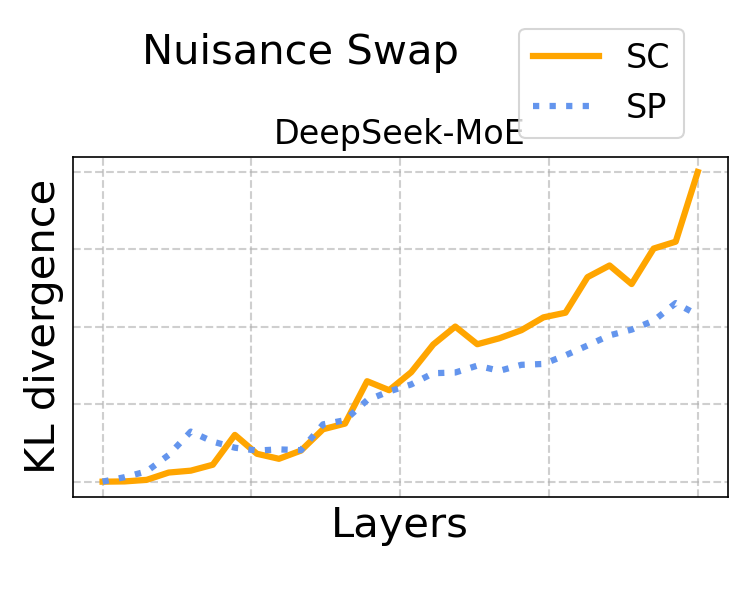
\includegraphics[width=0.58\linewidth]{figures/1_column_nuis_sc_sp_k32_group5.png}\\
\TinyCap{Single-group invariant-swap stress (Fig.~5 / Table~4).}

\vspace{0.15em}
\raggedright
Swap one component of the final-token hidden state; measure next-token KL.
{\scriptsize\color{AccentDeep}\textbf{Invariant swap}} keeps surface, replaces meaning;
{\scriptsize\color{Signal}\textbf{nuisance swap}} keeps meaning, replaces surface.
\textbf{Fig.~5:} SP donors barely move outputs; soft SC raises KL; between-group most.
\textbf{Fig.~6:} over 1{,}400 groups (95\% CIs), invariant KL $>$ nuisance KL at layers 3, 5, 8 (Table~16).
\end{block}

\begin{block}{Zero-shot model attribution}
Invariant-zone signatures identify the source model, including after fine-tuning
and distillation, and outperform PCA and cPCA with matched subspace size.

\vspace{0.25em}
\centering
\begin{tabular}{lccc}
\toprule
Variant & PCA & cPCA & Ours \\
\midrule
Base & 86.08 & 89.33 & \textbf{95.45} \\
Fine-tuned & 83.98 & 87.53 & \textbf{94.20} \\
Distilled & 81.25 & 84.65 & \textbf{92.25} \\
\bottomrule
\end{tabular}\\
\TinyCap{Fig.~8 / Table~6. Avg.\ over Llama, Mistral, Qwen2.5, Gemma.}
\end{block}

\begin{block}{Geometric separability (MS MARCO)}
\centering
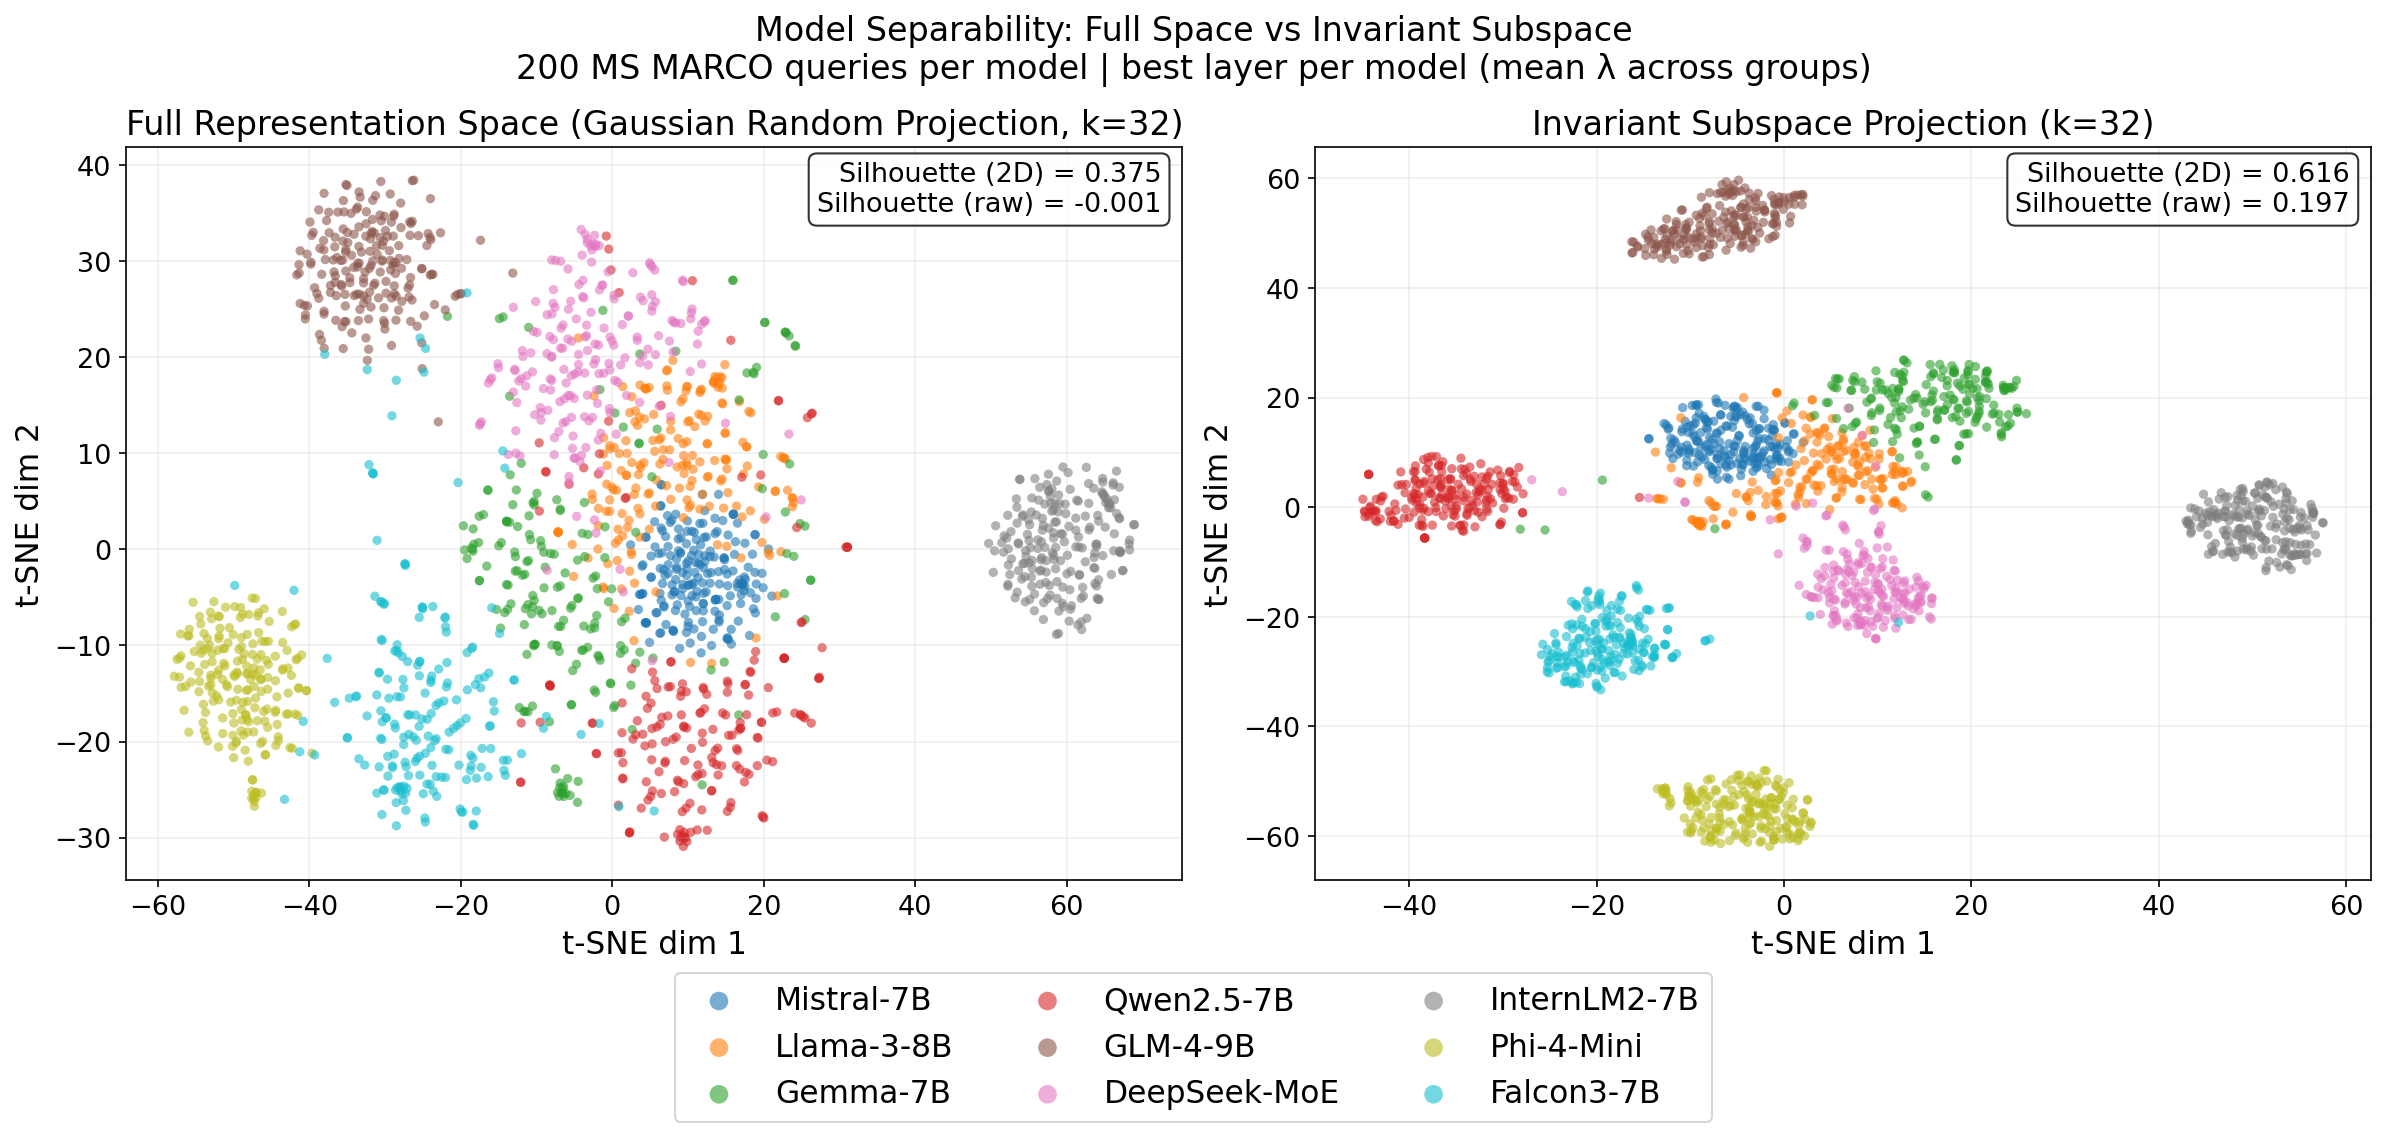
\includegraphics[width=0.90\linewidth]{figures/tsne_comparison_k32.png}\\
\TinyCap{Fig.~9. 200 MS MARCO queries/model ($k{=}32$). Left: full space. Right: invariant subspace.}
\end{block}

\begin{block}{Checks and limitations}
\textbf{Ambiguity:} lower $E_{\mathrm{nuis}}$ (layer~4: 0.0084 vs 0.0718 cPCA vs 0.0921 PCA).
\textbf{Multihop:} semantic vs nuisance KL 0.360 vs 0.069.
\textbf{Pooling / $k$:} last-token preferred; similar for $k\in\{1,10,32\}$.
{\scriptsize Limitations: local approx.; synthetic English; nuisance not fully disentangled.}
\end{block}

\vspace{0.1em}
\begin{minipage}{\linewidth}
\begin{minipage}{0.68\linewidth}
{\scriptsize\color{Muted}
Project: \href{https://cent664.github.io/LLMID/}{cent664.github.io/LLMID}\\
arXiv: \href{https://arxiv.org/abs/2605.06458}{arxiv.org/abs/2605.06458}\\[0.15em]
See project page for BibTeX.}
\end{minipage}\hfill
\begin{minipage}{0.28\linewidth}
\centering
\ProjectQR\\[-0.05em]
{\scriptsize\color{Muted}Project page}
\end{minipage}
\end{minipage}

\end{column}
\end{columns}

\end{frame}
\end{document}
